%!TEX root = ../Thesis.tex

\chapter{Selección de modelo} \label{ch:chap4}

\epigraphhead[70]{
\epigraph{Choose well. Your choice is brief, and yet endless.}
{Johann Wolfgang von Goethe}}

Puesto que el problema abarca también el detectar cuántos personas están involucrados en la grabación, y hasta ahora se ha considerado que se dispone de esta información, es necesario inferir de alguna manera cuántos interlocutores participan.

Si bien, una aparente desventaja del usar un \ac{HMM} como modelo es que se necesita saber a priori el número de estados que conforman la cadena (Fox~et~al.~\cite{Fox2011}), se propondrá un método para inferir cuál el el número correcto de estados en la cadena de Márkov.

La contribución principal de este trabajo de tesis está en la selección de modelo propuesta, utilizando varias técnicas tanto bayesianas como frecuentistas para respaldar la elección realizada.

Como mencionan Claeskens y Hjort \cite{Claeskens2010}, hay varios aspectos importantes que considerar antes de abordar el problema de selección de modelos: 

\begin{description}
\item[Los modelos son aproximaciones:] Cuando se usan modelos, se tiene que considerar que la realidad observada suele ser mucho más compleja que los modelos propuestos. No necesariamente existirá un modelo correcto 

\item[Sesgo-Varianza:] Se refiere a balancear tanto la simplicidad del modelo (pocos parámetros a estimar, lo que implicaría una menor variabilidad, aunque con cierto sesgo) contra la complejidad (introducir más parámetros al modelo reduciría el sesgo al modelar, pero aumentaría el grado de variabilidad). La selección estadística de modelos debe buscar un balance entre el sobre-ajuste (un modelo con muchos parámetros, más de los necesarios) o sub-ajuste (un modelo con muy pocos parámetros, no capture).

\item[Parsimonia:] 'El principio de parsimonia' o navaja de Ockham dice que 'en igualdad de condiciones, la explicación más sencilla suele ser la correcta'. Se puede pensar como incluir en el modelo sólo los parámetros que realmente importen y capturen la esencia del fenómeno. 

\item[Contexto:] Todo modelado tiene cierto propósito. Se pueden tener diferentes intereses para un mismo experimento, por lo que entonces el contexto no tiene que ser siempre el mismo para un conjunto de datos. En algunos contextos puede ser más interesante encontrar los parámetros subyacentes del modelo e interpretarlos, mientras que en otros puede bastar con obtener respuesta a las problema planteado.

\end{description}

Con estas consideraciones, se presentarán varios conceptos importantes que se utilizarán al momento de seleccionar el modelo adecuado:

\section{Funciones de penalización}

Una estrategia sencilla para la selección de modelo es elegir el candidato con la más grande probabilidad dados los datos. 

Comparar directamente los valores máximos alcanzados de log-verosimilitud para diferentes modelos no siempre es un criterio lo suficientemente bueno para la comparación de modelos. Al incluirse más parámetros en un modelo, la máxima log-verosimilitud también aumentará, pues el modelo se sobre-ajustará; por lo que no siempre será la mejor elección. 

Escoger el modelo con la mayor log-verosimilitud equivaldría a siempre elegir el modelo con más parámetros; lo que puede significar que tiene un buen poder predictivo para los datos que se usaron de entrenamiento, pero que probablemente en pruebas con otros datos diferentes no tendrá un buen desempeño.

Para evitar esto, se han diseñado funciones de penalización que permiten 

Entre las más comunes, se encuentran por ejemplo el \acf{AIC} o el \acf{BIC}, que se encargan de selección de modelo a partir de la estimación de máxima verosimilitud de los datos, así como también penalizan el número de parámetros libres que necesita el modelo.

\subsection{BIC}

Cuando hay varios modelos candidatos, una estategia bayesiana se encargaría de seleccionar el modelo que a posteriori sea más probable. Este modelo puede ser identificado calculando la probabilidad posterior de cada uno de los modelos y luego seleccionando aquél modelo cuya probabilidad sea la mayor.

A continuación, se muestra la derivación matemática de BIC desarrollada por Claeskens~et~al.~\cite{Claeskens2010}, así como una aproximación numérica para esta función. 

Sean $\mathcal{M}_1, ..., \mathcal{M}_k$ los modelos propuestos, y sea $\mb{X} = \lbrace x_1, ..., x_n \rbrace $ el vector de datos observados. La probabilidad a posteriori para cada modelo se puede calcular como sigue: 
\begin{equation}
P(\mc{M}_j \,|\, \mb{X}) \equiv \frac{P(\mc{M}_j)}{f(\mb{X})} 
  \int_{\Theta_j} f(\mb{X} \,|\, \mc{M}_j, \theta_j) \pi(\theta_j \,|\, \mc{M}_j) d\theta_j
\label{eqn:4-1}
\end{equation}
donde $\Theta_j$ es el espacio de parámetros al que pertenece $\theta_j$. Además, $f(\mb{X} \,|\, \mc{M}_j, \theta_j)$ es la verosimilitud $\mc{L}_{j}(\theta_j)$ de los datos, dado al modelo $j$ y sus parámetros; mientras que $ \pi(\theta_j \,|\, \mc{M}_j) d\theta_j$ representa la densidad a priori de $\theta_j$ dado el modelo $\mc{M}_j$; 
$P(\mc{M}_j)$ es la probabilidad a priori para el modelo $j$-ésimo y $f(\mb{X})$ es la verosimilitud de los datos.

La verosimilitud incondicional de los datos se puede calcular como sigue: 
\begin{equation}
f(\mb{X}) = \sum_{j=1}^k P(\mc{M}_j) \lambda_{n, j}(y)
\label{eqn:4-2}
\end{equation}
donde 
\begin{equation}
\lambda_{n, j} = \int_{\Theta_j} \mc{L}_{n, j}(\theta_j) \pi(\theta_j \,|\, \mc{M}_j) d\theta_j.
\label{eqn:4-3}
\end{equation}

La ecuación \eqref{eqn:4-3} representa la verosimilitud marginal de los datos para el modelo $\mc{M}_j$ integrada con respecto a $\theta_j$ sobre es espacio de parámetros $\Theta_j$ correspondiente.

Al comparar las probabilidades posteriores $P(\mc{M}_j \,|\, \mb{X})$ de los distintos modelos, $f(\mb{X})$ se mantiene constante para todos los modelos, por lo que se puede descartar en la comparación.

Ahora, si se define 
\begin{equation}
BIC_{n, j}^{exact} \equiv 2 log(\lambda_{n, j}(\mb{X}))
\label{eqn:4-4}
\end{equation}
por lo que \eqref{eqn:4-1} se podría reescribir como sigue: 
\begin{equation}
P(\mc{M}_j \,|\, \mb{X}) = \frac{ P(\mc{M}_j)  exp(\frac{1}{2} BIC_{n, j}^{exact}) }
{ \sum_{i=1}^k  P(\mc{M}_i) exp(\frac{1}{2} BIC_{n, i}^{exact}) }
\label{eqn:4-5}
\end{equation}

Sin embargo, el cálculo de los diferentes $BIC_{n, j}^{exact}$ es difícil de estimar numéricamente, además de que la expresión necesita las probabilidades a priori para todos los modelos y todos los parámetros; por lo que se buscará una expresión similar que sea práctica y mucho más eficiente.

Para esto, primero hay que considerar el método de Laplace, que es usado para aproximar integrales de la forma $\int_a^b e^{M f(x)} dx$, por lo que \eqref{eqn:4-3} debe escribirse de esa manera: 
\begin{equation}
\lambda_{n, j}(\mb{X}) = \int_{\Theta} exp\left\lbrace n h_{n, j}(\theta) \cdot \pi(\theta \,|\, \mc{M}_j) \right\rbrace ~d\theta 
\label{eqn:4-6}
\end{equation}
donde $h_{n, j}(\theta) = n^{-1} \ell_{n, j}(\theta)$ y $p = \#\theta$ es la cardinalidad del $\theta$; por lo que ahora usando la aproximación básica de Laplace, se tiene: 
\begin{equation}
\begin{split}
 &\int_{\Theta} exp \left\lbrace n h_{n, j}(\theta) \cdot \pi(\theta \,|\, \mc{M}_j) \right\rbrace ~d\theta = \\
 & \quad\quad \left( \frac{2 \pi}{n} \right)^{\frac{p}{2}} \cdot exp \left\lbrace n h(\theta_0) \right\rbrace \cdot
 \left\lbrace g(\theta_0) \cdot \left| J(\theta_0) \right| ^{-\frac{1}{2}} + O(n^{-1}) \right\rbrace
\end{split}
\label{eqn:4-7}
\end{equation}
donde $\theta_0$ es el valor que maximiza la función $h(\cdot)$ y $J(\theta_0)$ es el negativo de la matriz Hessiana 
\begin{equation}
J(\theta) \equiv -\frac{\partial^2 h(\theta)}{\partial \theta \cdot \partial \theta^T}
\label{eqn:4-8}
\end{equation}
evaluada en $\theta_0$.

Hay que notar que esta aproximación es equivalente a \eqref{eqn:4-4} sólo cuando $h$ es una forma cuadrática negativa (como lo es una log-verosimilitud gaussiana) y cuando $g(\cdot)$ es constante. 

En este caso, tenemos que $h(\theta) = n^{-1} \ell_{n, j}(\theta)$ y que se maximiza con el \ac{MLE} $\hat \theta_j$ para el modelo $\mc{M}_j$. Por otra parte, se puede aproximar $J(\theta_0)$ como la matriz de información mutua, que se define en el capítulo 2 de \cite{Claeskens2010}.

\section{Bootstrap}

Bootstrap es una técnica estadística que nos permite tener noción sobre qué tan precisa es alguna medida muestral estimada. Este método permite aproximar la distribución de muestreo de casi cualquier estadístico, usando métodos simples aunque computacionalmente intensivos. 

Como menciona Persi~et~al.~\cite{Diaconis1983}, esta técnica fue desarrollada en 1978 por Efron~\cite{Efron1978}, quien generalizó el método de \textit{Jacknife}; siendo ambos métodos estadísticos altamente demandantes en cuanto a procesamiento computacional; y que empezaron a tener más auge a finales de la década de 1970 debido al crecimiento del poder de cómputo disponible.

Una de las principales ventajas de esta técnica, de acuerdo a Burns~\cite{Burns2013}, es que no se asume que los datos con los se trabajarán tienen una distribución normal o alguna otra en específico; sino que al contrario, a partir de los observaciones se construirá su distribución empírica. Mientras mayor sea la cantidad de datos disponible, esta aproximación será mejor.

La técnica bootstrap se describe a continuación en un ejemplo: supongamos que se tiene que ajustar un modelo a un conjunto de datos. Sea este conjunto de entrenamiento $\mb{Z} = (z_1, z_2, ..., z_N)$ donde $z_i = (x_i, y_i)$ y son independientes con distribución $F$. Como $\mb{Z}$ es una muestra finita no se conoce tal cual la distribución $F$, pero se puede estimar una función empírica $\hat F$ donde a cada observación $z_i$ se le asigna un peso $\frac{1}{N}$ en la densidad.

Con esto, seleccionaremos de forma aleatoria y con reemplazo de $\hat{F}$ un conjunto de datos del mismo tamaño que el conjunto original. A este conjunto se le denotara $\mb{Z}^{*}_1$. Este proceso de selección se realiza $B$ veces, produciendo $B$ conjuntos bootstrap $\mb{Z}^{*}_{\cdot} = \lbrace \mb{Z}^{*}_1, \mb{Z}^{*}_2, ..., \mb{Z}^{*}_B \rbrace$. 

Luego, para cada uno de estos conjuntos, se volvera a ajustar el modelo, y se examinará el comportamiento de los ajustes para las respuestas obtenidas, obteniendo lo que se conoce como réplica bootstrap.

En \eqref{eqn:4-15}, $S(\mb{Z})$ representa cualquier estadístico calculado del conjunto de datos $\mb{Z}$. A partir de los conjuntos muestreados se puede estimar cualquier aspecto de una distribución de $S(\mb{Z})$, como por ejemplo, su varianza: 
\begin{equation}
\widehat{Var} \left[ S(\mb{Z}) \right] = \frac{1}{B-1} \sum_{b=1}^B \left( S(\mb{Z}^{*b}) - \bar{S}^{*} \right)^2
\label{eqn:4-15}
\end{equation}
donde $\bar{S}^{*} = \frac{1}{B} \sum_{b=1}^B S(\mb{Z}^{*b})$. Se puede pensar en $\widehat{Var} \left[ S(\mb{Z}) \right]$ como un estimador tipo Monte-Carlo para la varianza de $S(\mb{Z})$ a partir del muestro de la función de distribución empírica $\widehat{F}$ de los datos $(z_1, z_2, ..., z_n)$. De esta misma manera, se puede calcular la desviación estándar de otros estimadores de interés, tales como el coeficiente de correlación, algún cuantil, etc.

En la \autoref{fig:bootesq} se muestra el proceso general que se sigue para obtener las réplicas bootstrap \cite{Hastie2001}1.

\begin{figure}[tp]
  \centerline
  {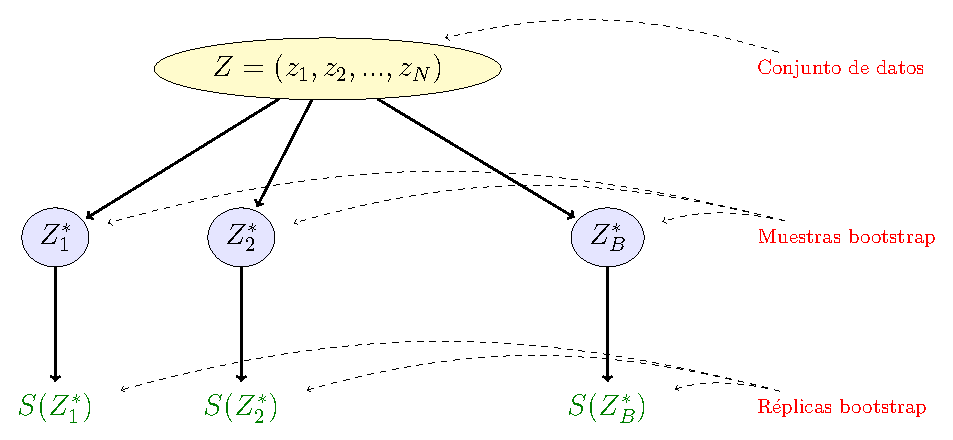
\includegraphics[width=1.1\linewidth]{gfx/chap4/untitled}}        
  \caption[Esquema del proceso bootstrap.]{Esquema del proceso bootstrap. Se desea estimar la precisión del estadístico $S(\mb{Z})$. Para esto, se generan $B$ conjutos, cada uno muestreando con reemplazo $N$ elementos del conjunto original. A cada uno de estos $b = 1, 2, ..., B$ elementos se le denomina $\mb{Z}^{*}_b$, y es a partir de estos que se calcula el estadístico de interés. Usando estas réplicas bootstrap es como se estima la varianza del $S(\mb{Z})$ previamente calculado.}
  \label{fig:bootesq}
\end{figure}

Hay que observar que lo que hace bootstrap es realmente estimar la varianza muestral a partir de la distribución empírica $\hat F$ y conforme $B \rightarrow \infty$, $\widehat{Var}(\hat F)$ tiende a la varianza poblacional $\widehat{Var}(\hat F) = {Var}(\hat F)$ de la misma $\hat F$. Para que realmente $\widehat{Var}(\hat F)$ converja a  ${Var}(F)$ se necesita además que $N \rightarrow \infty$, es decir, que se tengan muestras infinitas de la distribución original.

El ejemplo anterior, así como la mayor cantidad de literatura disponible tratan sobre bootstrap como una técnica para estimar errores estándar o construir intervalos de confianza de un estadístico \cite{MacKinnon2007}. Sin embargo, en este caso se usará bootstrap para realizar pruebas de hipótesis de una cola, fijando un nivel de significancia $\alpha$ que más adelante se especificará.

\subsection{Bootstrap paramétrico}

Como ya se mencionó, el bootstrap clásico es no paramétrico, y se vale únicamente del conjunto observado para a partir de ahí estimar la función de distribución empírica. En el caso que nos interesa, se cuenta con un modelo paramétrico que ha sido ajustado a los datos, usualmente por \ac{MLE}. 

Entonces, a partir de este modelo ajustado es que se muestrea. Al igual que en con la técnica no paramétrica, se suelen generan muestras de datos del mismo tamaño que el conjunto original. Luego, para cada nueva conjunto bootstrap $\mb{Z}^{*}_b$ muestreado se calcula el estadístico de nuestro interés. Éste proceso de muestreo se repite igualmente una gran cantidad de veces. 

El método de bootstrap paramétrico se suele utilizar en problemas en los que se desea ajustar un modelo y además encontrar sus parámetros correspondientes. Nos permite ajustar de mejor forma los parámetros de un modelo, calculando algún estadístido de interés que permita analizar el comportamiento de cada uno de los parámetros estimados.

\section{Selección de modelo usando BIC}

Como ya se mencionó al principio de este capítulo, hay muchas formas de aboradar el problema de selección de modelo. En este trabajo se usará una combinación de los dos tipos presentados.

Puesto que consideramos que dentro de nuestro espacio de modelos propuestos se encuentra el modelo solución (esto es, hay un modelo que corresponde con el número de interlocutores que participan en la grabación), resulta más natural usar \ac{BIC}.

Esta función de penalización se calcula de la siguiente manera: 
\begin{equation}
BIC(\mc{M}) = 2 \mc{L}_{max}(\mc{M}) - (log N ) dim(M)
\end{equation}
para cada propuesta de modelo $\mc{M}$, donde $dim(M)$ es el número estimado de parámetros libres que le corresponden, y $N$ es el tamaño de nuestra muestra de datos. Por otra parte, $\mc{L}_{max}(\mc{M})$ es la máxima log-verosimilitud obtenida para el modelo $\mc{M}$ después de realizar un número $K$ se simulaciones, para evitar que en algún caso el algoritmo de estimación se quede atorado en un máximo local.

Para estimar el número de parámetros libres de nuestro modelo, se consideran todas las probabilidades que rigen al \ac{HMM}, que en este caso son: la matriz a priori o inicial, la matriz de transiciones entre los interlocutores, así como la matriz de emisión de cada persona para todo el diccionario de palabras.

Este tipo de función de penalización nos permite seleccionar de entre un conjunto de modelos propuestos (que pueden ser muchos) al modelo o los modelos con mayor probabilidad de ser los correctos. 

Se enfoca en escoger el modelo candidato con la mayor probabilidad dados los datos, pero penalizando la complejidad de cada propuesta. Se preferirán entonces los modelos con una mayor verosimilitud que involucren la menor cantidad de parámetros posibles. 

En caso de que dos o más modelos tengan una puntaje similar en \ac{BIC}, se buscará hacer un análisis más extenuante para revisar cuál modelo es más conveniente.

\section{Selección de modelo usando bootstrap con likelihood ratio testing}

Para esta otro propuesta, se utilizará la técnica bootstrap paramétrico, pues mediante el algoritmo \ac{EM} es fácil obtener el modelo parametrizado. El estadístico a evaluar será el \ac{LLR}, que nos permitirá comparar entre dos modelos propuestos. 

Usualmente se compararán dos modelos adyacentes, es decir, el modelo $\mc{M}_d$ de $d$ estados contra el modelo $\mc{M}_{d+1}$ de $d+1$ estados ocultos.

La prueba que se realiza es comparando el \ac{MLE} $\hat \theta^{(d)}$ y $\hat \theta^{(d+1)}$ de los modelos de $d$ y $d+1$ estados respectivamente. Para la comparación se usa la estadística \ac{LLR} que corresponde a la diferencia de las log-verosimilitudes mencionadas
\begin{equation}
  LLR^{(d)}_{obs} = log \frac{L(\hat \theta^{(d+1)}; y_{1:n})}{L(\hat \theta^{(d)}; y_{1:n})} =
    log L(\hat \theta^{(d+1)}; y_{1:n}) - 
    log L(\hat \theta^{(d)}; y_{1:n})
\end{equation}

Para calcular el \ac{MLE} de un modelo, se estimó la verosimilitud varias veces con diferentes parámetros iniciales aleatorios. Se iteró el algoritmo \ac{EM} hasta convergencia, un numero $iter_{hmm}$ fijo de iteraciones, esto para evitar el estancamiento del algoritmo en un máximo local, y obtener así una buena estimación de la máxima verosimilitud del modelo.

Se usó entonces como \ac{MLE} del modelo la máxima verosimilitud correspondiente a los mejores parámetros estimados y que se denotó por $LLR_{obs}$.

Ahora, para hacer la prueba con bootstrap se simularán datos de los \ac{HMM} propuestos, utilizando el algoritmo \ref{alg:ancsamp} para el muestreo, tanto para el modelo $\mc{M}_d$ como para el modelo $\mc{M}_{d+1}$. Para ambos modelos se estimará su log-verosimilitud y se procederá con el cálculo del \ac{LLR}, que es la réplica bootstrap que nos interesa. 

\begin{algorithm}[tp]
   \caption{Muestreo ancestral para un HMM}
   \label{alg:ancsamp}
\begin{algorithmic}
   \STATE {\bfseries Input:} \\
   núm. de estados $N$, núm. de muestras en el tiempo $T$ \\
   núm. de posibles valores en el diccionario $K$, \\
   $ \pi \in \mathcal{R}^{N}; ~~ \pi_j = p(z_{1j})$ \\
   $ \mathbf{A} \in \mathcal{R}^{N \times N}; ~~
   \mathbf{A}_{jk} = p(z_{nk} \,|\, z_{n-1, j})$ \\

   $ \mathbf{B} \in \mathcal{R}^{K \times N}; ~~
   \mathbf{B}_{jk} = p(x_{nk} \,|\, z_{n, j})$\\  
   \STATE
   \STATE $z_1 \sim Multinomial(\pi)$   
   \STATE $x_1 \sim Multinomial(\mathbf{E}_{[z_1,~:]})$

   \FOR{$i = 1 \to T$} 
    \STATE $z_t \sim Multinomial(\mathbf{A}_{[z_{t-1},~:]})$ 
    \STATE $x_t \sim Multinomial(\mathbf{B}_{[z_t,~:]})$
   \ENDFOR   
\end{algorithmic}
\end{algorithm}

Para cada par de modelos $\mc{M}_d, \mc{M}_{d+1}$ se realizará este procedimiento $B$ veces: muestreando ambos modelos, estimando su verosimilitud y calculando el estadístico $\ac{LLR}$. Para cada simulación bootstrap se generará un $LLR_{boot}^b$ referente a la muestra generada. 

Cuando se termine el proceso bootstrap, se tendrán $\lbrace LLR_{boot}^b \rbrace_{b=1}^B$ estadisticos, y se podrá generar una densidad sobre los valores de $LLR_{boot}^b$. 

La última etapa será realizar una prueba de hipótesis para ver si el valor $LLR_{obs}$ tiene la misma distribución que los $\lbrace LLR_{boot}^b \rbrace_{b=1}^B$. La hipótesis nula será que el modelo $\mc{M}_d$ es el modelo correcto, y entonces el valor $LLR_{obs}$ estará en el rango mismo de los $LLR_{boot}$. Sin embargo, si se rechaza la hipótesis nula (de acuerdo a un nivel de significancia establecido) significará que el modelo $\mc{M}_{d+1}$ es mejor que el $\mc{M}_{d}$.